% -*- root: ../main.tex -*-
%!TEX root = ../main.tex
% this file is called up by main.tex
% content in this file will be fed into the main document
% vim:textwidth=80 fo=cqt

\graphicspath{{chapters/dra/figures/}}
% ----------------------- contents from here ------------------------

\chapter{Computational Analysis and Numerical Reformulation of the \glsfmtshort{dra}}\label{ch:improveddra}
% \chapter{Analysis of the \glsfmtlong{dra} and Performance Boost through Numerical Reformulation}\label{ch:improveddra}
% \chapter{Computational Bottleneck Analysis of the \glsfmtshort{dra} and its Mitigation through Numerical Reformulations}\label{ch:improveddra}
\vspace*{-1em}
\startcontents[chapters]
\printcontents[chapters]{}{1}{\setcounter{tocdepth}{1}}

% \bigskip

\capolettera{T}{his} chapter presents  an analysis and critical  evaluation of a
computational bottleneck present in  a popular physics-based \gls{rom} framework
of lithium-ion batteries and proposes  an alternative numerical reformulation to
mitigate  it\footnote{This  chapter is  based  on  the journal  publication  ---
\fullcite{Gopalakrishnan2017}.  All  intellectual  ideas in  the  aforementioned
article  are original  contributions of  this thesis  author. All  text, tables,
figures  and captions  therein were  contributed solely  by this  thesis author.
Copyright  clearance for  non-commercial  verbatim reproduction  of the  content
(such as in this thesis) has been secured through the publication agreement with
the  copyright holder  ASME (see  \cref{ch:permissions}). The  contents in  this
chapter may be, in full or in part, included verbatim from the said publication.
This  author wishes  to express  his thankfulness  to Teng  Zhang, co-author  of
this  article, for  checking  my calculations  and  providing valuable  feedback
that  helped to  refine  the  manuscript for  that  journal publication.}.  From
the  literature review  presented in  \cref{ch:littreview}, it  may be  recalled
that  transcendental  transfer functions  of  the  cell's electrochemical  field
variables  (except for  ionic concentration  and potential  in the  electrolyte)
was  obtained  by  Smith~\etal~\cite{Smith2007}  through  linearisation  of  the
underlying \gls{p2d} model equations. Lee~\etal~\cite{Lee2012a,Lee2012} extended
the aforementioned approach  so as to obtain  these missing electrolyte-specific
transfer  functions through  a multi-modal  EigenFunction expansion  employing a
Sturm-Liouville approach~\cite{Pryce1993}.


In order to arrive at a  \gls{lti} state-space representation of the system (see
\cref{eq:LTIstatespace})  for embedded  implementation, Lee~\etal{}  devised the
\gls{dra}, a numerical procedure  to systematically transform all transcendental
transfer functions  to the time domain.  A special property of  the \gls{dra} is
that it  retains the physical nature  of the original \gls{dfn}  equations until
the very  last step  wherein the  matrices governing  the system's  dynamics are
generated. This  yields a  one-dimensional discrete-time  \gls{rom} of  the cell
that is entirely based upon  fundamental physical principles. The \gls{rom} thus
obtained could  then be used to  compute the time-evolution of  all the internal
electrochemical quantities of  the \gls{dfn} model. Prima~facie  it appears that
this model  could be directly  implemented for embedded  vehicular applications,
for  example,  as  the  plant  model for  state  estimation  tasks.  However,  a
comprehensive analysis  of the procedure reveals  a critical issue that  must be
first tackled before implementation aspects can be considered.

The  unresolved  issue in  Lee~\etal{}  is  the excessively  high  computational
requirements associated with the \gls{dra}, which becomes a crippling bottleneck
since  the  procedure  needs  to   be  repeated  for  multiple  \glspl{soc}  and
temperatures.  This  computational  bottleneck   arises  from  forming  a  large
Block-Hankel  matrix  in memory  upon  which  a  \gls{svd} is  performed.  Under
certain conditions  as discussed in  \cref{sec:size-of-the}, owing to  the large
size  of  the  Block-Hankel  matrix,   the  \gls{dra}  computation  is  rendered
intractable. This issue has been acknowledged by the original authors themselves
in~\cite{Lee2012,Plett2015}.  In  this  chapter, this  computational  bottleneck
is  analysed  and an  improved  scheme  is proposed.  \Cref{sec:Analysis-of-the}
discusses an analytical evaluation of  the massive computing requirements of the
original  \gls{dra} method.  Redundancies and  inefficiencies in  this step  are
enumerated  and the  high  computational  costs are  deemed  as unnecessary.  In
\cref{sec:Efficient-Computation-of}, a fast  computational approach is presented
which  significantly reduces  both  the  memory and  computational  time of  the
\gls{rom}  workflow. \Cref{sec:Results}  summarises  the  results obtained  from
applying the  new workflow presented in  \cref{sec:Efficient-Computation-of}, by
comparing and contrasting the much smaller computational requirements of the new
method  with the  original  \gls{dra} scheme.  The  improved modelling  accuracy
achieved  by  this  proposed  method when  deployed  under  resource-constrained
computing environments, is also highlighted.

\section{Analysis of the Computational Bottlenecks of the \glsfmtshort{dra}}\label{sec:Analysis-of-the}

The \gls{rom}  proposed by  Lee~\etal{} aims  for the  simplified representation
of  the  \glsfirst{p2d}  volume-averaged  continuum  model  proposed  by  Doyle,
Fuller   and   Newman~\cite{Doyle1993a,Fuller1994}\footnote{hereafter   referred
    interchangeably in  this thesis  by the two  acronyms ---  \glsfmtshort{dfn} and
\glsfmtshort{p2d}.}.


The   block   diagram   in  \cref{fig:traditional_ROM_Workflow}   depicts   this
thesis  author's   summary  presentation  of  the   overall  modelling  workflow
in   Lee~\etal{}.   Firstly,  the   governing   \gls{pdae}   equations  of   the
\gls{dfn}   model    (see   \cref{tbl:dfneqns})   are   linearised    about   an
operating  point  of  \gls{soc}   and  temperature.  Then,  closed-form  Laplace
domain  transcendental   transfer  functions   of  all  the   internal  physical
quantities~$\left(\phi_{s},\phi_{e},c_{s},c_{e},j\right)$   at  different   cell
locations, are derived using applied current  as the input. A detailed treatment
of  this analytical  derivation is  presented in  Lee~\etal~\cite{Lee2012a}. The
authors  proposed  a novel  \glsfirst{dra}  scheme~\cite{Lee2012b}  in order  to
transform  these  transcendental  transfer  functions  to  standard  state-space
representation.  Sublevel-1   of  \cref{fig:traditional_ROM_Workflow}   shows  a
breakout view of  the \gls{dra} procedure and illustrates the  steps involved in
this  computation. At  the  heart  of this  numerical  method  is the  classical
subspace  identification approach  known as  Ho-Kalman algorithm~\cite{HO1966a},
whose  computation steps  are  shown  via the  exploded  view  in sublevel-2  of
\cref{fig:traditional_ROM_Workflow}.  Then,  the Markov  parameters  (unit-pulse
response) of  this \gls{simo}  linear system of  battery transfer  functions are
computed\footnote{A  ubiquitous concept  in linear  systems and  control theory,
Markov parameters  represent the discrete-time  unit pulse response of  a linear
system.}.  They  form the  entries  of  a Block-Hankel  matrix~\cite{Ljung1998},
wherein each block  element is a column  vector of the set  of Markov parameters
at  a  given  time-step.  A  key  computation  in  the  Ho-Kalman  algorithm  is
the  \glsfirst{svd}  of this  Block-Hankel  matrix.  A  wide separation  in  the
magnitude  drop  between  successive  singular  values serves  as  a  guide  for
the  modeller in  choosing  a suitable  reduced order  to  represent the  entire
dynamics  of  the  system.  The   analyses  of  this  thesis  author,  presented
in \cref{subsec:Traditional-DRA--Memory}  and \cref{subsec:Traditional-DRA--CPU}
reveal major inefficiencies in both the Block-Hankel formation and the \gls{svd}
computation steps which hinder the entire reduced-order modelling workflow.

\begin{figure}[!htbp]
    \centering
    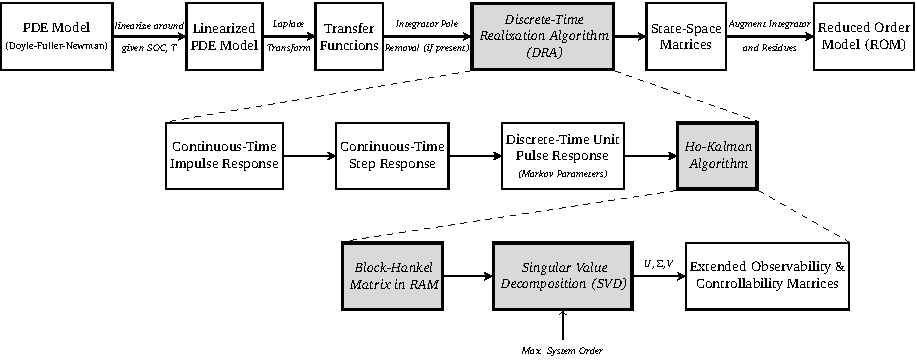
\includegraphics[width=\textwidth]{traditional_dra.pdf}
    \caption[%
    \glsfmtshort{rom} workflow using classical \glsfmtshort{dra}.
    ]%
    {%
        \glsfirst{rom} workflow using classical
        \glsfirst{dra}. The shaded blocks represent computational bottlenecks.
    }%
    \label{fig:traditional_ROM_Workflow}
\end{figure}

\subsection{Size of the Block-Hankel Matrix}\label{sec:size-of-the}

Large Block-Hankel matrices can occur in \gls{dra} computation due to the
following reasons.
\begin{enumerate}
    \item
        For  a  given   duration  of  Markov-parameter  recording,   if  a  high
        sample-rate   \gls{rom}  is   desired,   the   emulation  frequency   in
        the   \gls{dra}  scheme   has   to  be   proportionately  increased   to
        accurately  compute  the continuous-time  step  and  pulse responses  in
        \cref{fig:traditional_ROM_Workflow}. This implies  that the total number
        of time-samples~$N$  for each  Markov parameter will  have to  be scaled
        linearly to  capture the  desired duration  of the  unit-pulse response.
        However,  the size  of the  Block-Hankel matrix  has a  \emph{quadratic}
        dependence on the Markov parameter length.
    \item
        The  recorded sample  size~$N$ could  also  become large  if the  Markov
        parameters of just  one of the transfer functions decay  very slowly. In
        Li-ion batteries, diffusion  within the solid particle  is typically the
        slowest process.  For the cell  modelled in Lee~\etal{},  the unit-pulse
        response of surface concentration of Li adjacent to the positive current
        collector  requires approximately  16000~samples before  reducing to  an
        appreciably low value, as shown in \cref{fig:markov_cse_pos}.
    \item
        For  a  battery  modelling   problem  consisting  of  multiple  transfer
        functions,  the  number  of  entries in  the  Block-Hankel  matrix  also
        scales linearly  with the  number of transfer  functions. Thus,  if more
        cell  variables (\eg~concentrations and  potentials at  other spatial
        locations  within the  cell) are  to be  studied, then  the size  of the
        transfer function vector  and that of the  Block-Hankel matrix increases
        correspondingly.
\end{enumerate}

\begin{figure}[!htbp]
    \centering
    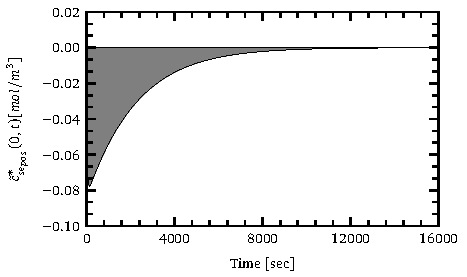
\includegraphics{markov_decay.pdf}
    \caption[Markov parameters of solid surface concentration at positive
    current collector]{Time evolution of Markov parameters of pole-removed transfer
        function corresponding to surface concentration of Li in the solid particle
    adjacent to positive current collector.}
    \label{fig:markov_cse_pos}
\end{figure}

Considering the combined  influence of these effects,  if $x$~transfer functions
are  to be  modelled and  $N$~time-samples of  each Markov  parameter are  to be
captured, the corresponding size of the Block-Hankel matrix~$H$ is
\begin{equation}
    \text{Size}(H)\sim \mathcal{O}(x N^2)\text{ entries}
\end{equation}

This    has    a    significant     computational    impact    as    shown    in
\cref{subsec:Traditional-DRA--Memory} and \cref{subsec:Traditional-DRA--CPU}.

\subsection{Classical \glsfmtshort{dra} --- Memory (\glsfmtshort{ram}) Requirements}\label{subsec:Traditional-DRA--Memory}

Lee~\etal~\cite{Lee2012a}  modelled 28~transfer  functions representing  various
electrochemical  variables at  the current  collector and  separator interfaces.
Each Markov  parameter is  a 28~element  column vector.  16000~time-samples were
obtained at  a sample-rate of  \SI{1}{\hertz}, allowing sufficient time  for the
Markov parameters  of the  slowest dynamics  \ie~solid surface  concentration to
settle  to an  acceptably low  magnitude.  The Block-Hankel  matrix thus  formed
has  8000~blocks, each  block  consisting of  28~elements  \ie~has $8000  \times
28=224000$~rows  and 8000~columns.  Hence,  the overall  number  of elements  in
the  Block-Hankel matrix  is~${224000  \times 8000=1.79  \times 10^{9}}$.  Using
double-precision  arithmetic, its  storage requirement  can be  estimated to  be
\approx \SI{27}{\giga\byte}.

Computing the \gls{svd} results in the formation of three more large matrices in
memory ---
\begin{enumerate*}[label=\roman*)]
    \item matrix   of   output  singular   vectors~$U$,
    \item matrix of  input  singular vectors~$V$, and
    \item the diagonal singular-value  matrix~$\Sigma$.
\end{enumerate*}
With  8000~Hankel-blocks,  approximately  \SI{81}{\giga\byte}  of  \gls{ram}  is
required for holding these three output  matrices generated by a full \gls{svd}.
However,  the  intermediate  operational   memory  usage  during  the  \gls{svd}
computation is often much higher than the  combined size of all the matrices. As
these large  matrices must  be repeatedly  handled for  each operating  point of
\gls{soc} and  temperature, the  high memory demand  of the  classical \gls{dra}
remains a persistent issue.

\subsection{Classical \glsfmtshort{dra} --- \glsfmtshort{cpu} Operation Count}\label{subsec:Traditional-DRA--CPU}

The most widely  used numerical algorithm for computing the  full \gls{svd} of a
generic dense matrix~${\ensuremath{A\in\mathbb{R}^{m \times n},m\geq n}}$ is the
two-stage  Golub-Kahan-Reinsch  method~\cite{Golub2013}.  In  the  first  stage,
${A\in\mathbb{R}^{m \times n}}$~is  reduced to an upper bidiagonal  form. In the
second  stage, \gls{svd}  of  this  upper bidiagonal  matrix~${B\in\mathbb{R}^{m
\times   n}}$  is   computed  using   an   iterative  procedure   such  as   the
Demmel-Kahan method~\cite{Golub2013}. If  stage~\romanletter{1} of the \gls{svd}
computation  employs~$\mathbb{R}$-Bidiagonalisation~\cite{Golub2013},  then  the
overall  process is  referred to  as~\mbox{$\mathbb{R}$-\gls{svd}}. This  is the
fastest known  full \gls{svd}  computation method  that may  be applied  to this
battery modelling problem. The \textsc{dgesvd} algorithm, originally implemented
in  \textsc{LAPACK}~\cite{Anderson1999},  employs  this method.  This  has  been
ported to  many numerical computation  packages such  as MATLAB, GNU  Octave and
Scilab.  Several  numerical  libraries  such  as NAG  and  Intel  MKL  also  use
the  \textsc{dgesvd}  codes  due  to its  acclaimed  stability,  robustness  and
versatility.  The MATLAB  implementation `\texttt{\textbf{svd}}'  is also  based
upon \textsc{dgesvd} and  hence this can be considered as  the de-facto baseline
\gls{svd} code.

The    operation    count    for    computing   the    singular    values    and
vectors    of    a    generic    dense    matrix~${\ensuremath{A\in\mathbb{R}^{m
\times   n},m\geq   n}}$    using   the   \mbox{$\mathbb{R}$-\gls{svd}}   method
is~${\ensuremath{4m^{2}n+22n^{3}}}$~\cite{Golub2013}.   Markov   parameters   of
$x$~transfer functions  and $N$~time-samples  yields a Block-Hankel  matrix with
$m=x N$~rows and $n=N$~columns. Hence,
\begin{alignat}{2}
    \text{\glsfmtshort{cpu} Operation  Count} & = & \,4\left(xN\right){}^{2}N+22N^{3}\nonumber \\
                                              & = & \,2N^{3}\left(11+2x^{2}\right)\label{eq:cpu_op_count}
\end{alignat}
Thus  the  \gls{cpu} operation  count  scales  as~${\mathcal{O}(N^{3})}$ with  the
number of Markov time-samples~$N$ and as ${\mathcal{O}(x^{2})}$ with the number of
transfer  functions~$x$ being  modelled. The  \gls{rom} computed  in Lee~\etal{}
uses  28~transfer functions  wherein  the Markov  parameters  are collected  for
\SI{16000}{\second}  with  a sampling  interval  of  \SI{1}{\second}. Thus,  the
\gls{cpu}  operation  count for  performing  this  computation is  approximately
${\mathcal{O}(16000^{3})\approx 4 \times 10^{12}}$~floating point operations.

\subsection{Summary Effect of Computational Bottlenecks}\label{subsec:Summary-Effect-of}

The computational bottleneck in a  classical \gls{dra} implementation arises due
to the  requirement of capturing a  large number of Markov  parameters, which in
turn leads  to growth in  Block-Hankel size. In  the case of  battery modelling,
this can arise in the following real-life scenarios:
\begin{enumerate}
	\item
        Electrochemical variables at additional locations of interest within the
        cell (\eg~middle of electrode or  separator domain) might need  to be
        modelled. This increases the number  of transfer functions and hence the
        number of Markov parameters.
	\item
        High frequency load  cycles necessitate higher sample-rates  to obtain a
        high fidelity  model. This leads  to a correspondingly higher  number of
        Markov parameters.
	\item
        In cells with  large particle sizes and small  diffusion coefficients, a
        large set  of Markov  parameters is  needed to  capture the  full system
        dynamics.
\end{enumerate}
Lack  of  specialised  computing infrastructure  necessitates  early  truncation
of  the  Markov parameters  in  the  \gls{rom}  workflow. The  resulting  errors
in  the singular  value  computation  lead to  significant  modelling errors  in
the  physical  variables of  the  cell.  Thus,  in practice,  the  computational
bottlenecks of classical \gls{dra} manifest as modelling errors when implemented
in  a  resource-constrained  computing environment.  Furthermore,  this  tedious
computation has to be repeated for multiple \glspl{soc} and temperatures.

The foregoing analysis  clearly demonstrates that the high  memory and \gls{cpu}
demands in  a classical \gls{dra}  implementation severely hamper the  scope and
applicability  of the  reduced order  modelling process.  This implies  that the
modelling  workflow is  not accessible  to research  groups without  specialised
computing infrastructure and its universal  appeal is rendered questionable. The
shaded  blocks in  \cref{fig:traditional_ROM_Workflow}  depict the  hierarchical
propagation of the classical \gls{dra}'s computational bottleneck throughout the
\gls{rom} workflow.

\section{Improved \glsfmtshort{dra} for Battery Modelling}\label{sec:Efficient-Computation-of}

Collecting a  large Markov parameter  set is  inevitable due to  the fundamental
physics of the cell  dynamics as established in \cref{subsec:Summary-Effect-of}.
Hence, in  order to circumvent the  high computational demands of  the classical
\gls{dra}, the second step in the process \ie~forming the Block-Hankel matrix,
is critically examined with the following scientific rationale.

\begin{enumerate}
	\item
        The unit-pulse responses of most  battery transfer functions (other than
        those of rate-limiting  steps such as solid  diffusion) decay relatively
        quickly. Hence it is inefficient to  record the Markov parameters of the
        full  system for  the  entire  duration needed  to  capture the  slowest
        dynamics.
	\item
        The Block-Hankel  matrix is essentially redundant  information since its
        entries are simply the Markov parameters arranged in a repeating special
        structure. Thus,  it is wasteful to  construct this huge matrix.  If the
        \gls{svd} operation  can be  performed on a  virtual Hankel  matrix, the
        memory requirements can be drastically reduced.
	\item
        The matrix of singular values~$\Sigma$ is diagonal and hence, sparse. It
        is redundant to hold all the non-diagonal entries (zeros) in memory.
	\item
        It  is not  necessary to  perform a  \emph{full} \gls{svd}  operation in
        order  to  achieve order  reduction.  When  an  upper bound  on  desired
        system order  can be  decided a  priori, it is  sufficient to  compute a
        \emph{truncated}  \gls{svd} yielding  the  first  few dominant  triplets
        of~${U, \Sigma \text{ and } V}$.
\end{enumerate}
Thus,  forming the  large Block-Hankel  matrix  and computing  its \gls{svd}  is
identified as an avoidable bottleneck in the classical \gls{dra}method. This can
be  tackled since  forming the  Block-Hankel matrix  is an  idiosyncrasy of  the
algorithm  used  and  does  not  arise from  any  fundamental  physical  limits.
Facilitated  by  an  efficient  \gls{svd}  implementation,  this  thesis  author
proposes  an improved  \gls{dra}that  serves  as a  drop-in  replacement in  the
\gls{rom} workflow.

\subsection{Candidate Schemes for Block-Hankel \glsfmtshort{svd}}

Generic  \gls{svd}  routines  such  as \textsc{dgesvd}  do  not  take  advantage
of  the  anti-diagonal  structural  symmetry  of  Block-Hankel  matrices.  Since
it  is sufficient  to  obtain  the first  few  leading  eigentriplets for  order
reduction,  iterative  algorithms  such  as   the  Jacobi  and  Lanczos  schemes
(see~\cite{Golub2013})  emerge  as  attractive candidates  for  computing  these
dominant singular  values and vectors. In  order to ensure accessibility  to the
large community of  battery researchers and to encourage  widespread adoption of
the fast reduced order modelling framework, the author of this thesis considered
only freely available  open-source numerical libraries that exist  in the public
domain, especially  those with permissive  licensing terms. Otherwise  the gains
achieved by  an efficient  \gls{svd} computation  for implementing  \gls{dra} on
non-specialised  computing  hardware would  be  offset  by commercial  licensing
terms,  usage restrictions  and  monetary considerations  associated with  using
proprietary  codes. Among  these  open-source candidate  algorithms, the  Jacobi
scheme~\cite{Golub2013} is  available through the  xGESVD routine in  the LAPACK
suite~\cite{Anderson1999}. FORTRAN 77 codes for the implicitly restarted Arnoldi
and Lanczos schemes~(see~nu-TrLan~\cite{Yamazaki2008}) are  available as part of
the ARPACK~\cite{Lehoucq1998} library.

The practical drawback  of most \gls{svd} implementations,  both open-source and
proprietary, is  that they require  the entire  matrix as input  argument. Since
operating upon  the Block-Hankel  matrix requires constructing  it in  the first
place, the memory bottlenecks discussed in \cref{subsec:Traditional-DRA--Memory}
are not  ameliorated. An  example is  the \texttt{svds}  routine ---  an economy
size  \gls{svd}  implementation  in  MATLAB\@.   Albeit  this  is  a  commercial
implementation  of  the  Arnoldi  codes,  any potential  benefits  of  using  an
iterative scheme is nullified by the memory penalty. Owing to reasons enumerated
in \cref{sec:Efficient-Computation-of}, the chosen  \gls{svd} algorithm needs to
be able to handle the computation without actually forming the huge block-Hankel
matrix in memory.

\subsection{\glsfmtshort{svd} Operation on a Virtual Block-Hankel Matrix}

The  pioneering  work  by  Larsen, PROPACK~\cite{LarsenPropack},  based  on  his
earlier work~\cite{Larsen1998} implements a numerically stable Lanczos \gls{svd}
computation designed specifically for large  and sparse matrices. In addition to
the ability  to operate on the  matrix as a  whole, the PROPACK codes  possess a
unique flexibility  of accepting  input arguments  in a  functional form.  A key
highlight of the  Lanczos \gls{svd} scheme is that it  does not strictly require
the  matrix  itself, but  only  the  product of  the  matrix  and its  transpose
with  an  arbitrary vector.  This  feature  has  been effectively  exploited  in
the  PROPACK suite.  Therefore, these  multiplication routines  can be  supplied
as  input  arguments instead  of  forming  the  large Block-Hankel  matrices  in
memory.  Furthermore,  this  package  includes  sophisticated  schemes  such  as
Gram-Schmidt  partial re-orthogonalisation~\cite{Bjorck1994}  to compensate  for
numerical round-off  errors in the  basic Lanczos bidiagonalisation  and ensures
orthogonality of  the input and  output singular  vectors. The PROPACK  suite is
available as both Fortran~77 and MATLAB codes distributed under a permissive BSD
license. Version~1.1 of the MATLAB implementation  of the PROPACK suite was used
by this thesis author.

For the \gls{rom} workflow, in order  to use PROPACK's unique feature \viz~its
flexibility to  accept functional form  inputs, the key  is to use  an algorithm
that  effectively  exploits the  affine  structure  of the  Block-Hankel  matrix
without  actually  forming  it  in  memory. Recent  research  in  a  specialised
time-series technique known as \gls{ssa}~\cite{Elsner1996} has yielded efficient
methods for  achieving this goal.  Korobeynikov~\cite{Korobeynikov2010} proposed
an  algorithm that  employs the  \gls{fft} for  implementing this  matrix-vector
product  by  embedding the  Markov  parameters  into  the  column vectors  of  a
circulant  matrix.  This  is  suitable   for  applications  wherein  the  Hankel
matrix  is  composed  of scalar  entries  such  as  that  formed by  the  Markov
parameters  of   a  \gls{siso}   transfer  function.  Golyandina,   Usevich  and
colleagues~\cite{Golyandina2010,Golyandina2015}  extended  this  approach  to  a
generic  2D-case for  performing \gls{ssa}  on images.  With this  modification,
this  algorithm is  rendered capable  of handling  the structure  of Multi-level
Block-Hankel matrices formed from the  Markov parameters of a generic \gls{mimo}
system. While  the modified  scheme does not  construct the  Block-Hankel matrix
in  memory,  the operational  rubrics  of  the Golyandina-Usevich  algorithm  in
conjunction with  PROPACK is  such that  they iteratively  operate on  a virtual
Hankel matrix  of equivalent size.  The Golyandina-Usevich algorithm  is briefly
summarised in \cref{sec:Golyandina-Usevich-Algorithm}.

\section{Golyandina-Usevich Algorithm\label{sec:Golyandina-Usevich-Algorithm}}

The  Golyandina-Usevich  algorithm  is  used  for computing  the  product  of  a
Block-Hankel matrix with an arbitrary vector.  The steps involved in this scheme
are enumerated  in Algorithm~3 of  Golyandina~\etal~\cite{Golyandina2015}. These
steps are reproduced  here in the context of the  improved \gls{dra} for reduced
order battery modelling.

\begin{enumerate}
	\item Compute a 2-D \gls{fft} of Markov parameter matrix.
	\item Form an augmented vector by zero-padding the arbitrary vector input
	    from Lanczos iteration.
	\item Perform a column-wise reshaping of this augmented vector to obtain
	    a new matrix with the same dimensions of the Markov parameter matrix.
	\item Compute the element-wise product of this newly created matrix with
	    the 2-D \gls{fft} of Markov parameter matrix.
	\item Reshape the resulting matrix back to a column vector.
	\item Extract the first $L$~elements from this vector, wherein~${L=K x}$.
	    $K$~represents the desired block-Hankel size and $x$~represents
	    the number of transfer functions being modelled.
\end{enumerate}

At the end of  Step~6, the product of the Hankel matrix  and arbitrary vector is
obtained. This is  reused as an input  for the Lanczos scheme  which generates a
new arbitrary vector  in the subsequent iteration. Thus, the  steps 1--6 are run
in a loop within the main Lanczos scheme.  These same steps can also be used for
computing the  product of the transpose  of the Hankel matrix  and the arbitrary
vector.  The only  change is  to  account for  the different  dimensions of  the
arbitrary  vector input  from  the  Lanczos scheme  in  step~2.  As a  practical
implementation, software code representing steps 1--6 is written in a plain-text
file and used  as functional-form inputs by the PROPACK  scheme which implements
the Lanczos iteration.

\section{Customisations for Battery Modelling}

Specific considerations  are required  for incorporating  the Golyandina-Usevich
algorithm  in  the  \gls{rom}  workflow  for  Li-ion  batteries.  The  classical
\gls{dra}  architecture is  set up  to  handle \gls{simo}  systems, wherein  all
transfer functions  are derived by  considering only  a single input  \viz~the
applied battery  current. Thus  the Markov parameters  form a  2D~matrix wherein
each  row corresponds  to  individual battery  transfer  functions with  columns
representing  unit-pulse  response  samples  for  each  transfer  function.  The
2D~moving-window  illustrated in~\cite{Golyandina2015}  for Block-Hankel  matrix
formulation has to be suitably reshaped to account for this structure. Step~3 of
the  algorithm  deals  with  2-D~\gls{fft}  computation  of  the  \gls{mpm}.  In
this  thesis author's  implementation,  this is  pre-computed  since it  remains
invariant between iterations of the Hankel-vector product computation loop. This
pre-allocation and a~priori computation contributes to overall code efficiency.


\begin{figure}[!htbp]
    \centering
    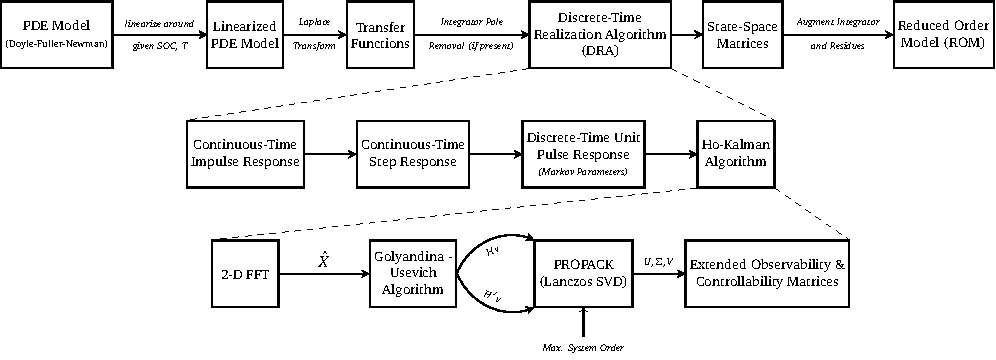
\includegraphics[width=\textwidth]{new_rom.pdf}
    \caption[%
    \glsfmtshort{rom} workflow using improved \glsfmtshort{dra}
    ]%
    {%
        \glsfirst{rom} workflow using improved \glsfirst{dra}.
    }%
    \label{fig:improved_ROM_workflow}
\end{figure}

\Cref{fig:improved_ROM_workflow} shows the \gls{rom}  workflow with the improved
\gls{dra} wherein all computational bottlenecks  highlighted by shaded blocks in
\cref{fig:traditional_ROM_Workflow}  have been  eliminated. The  strategy is  to
first employ the (suitably modified) Golyandina-Usevich algorithm for describing
the matrix-vector  multiplication routines.  These two  functions are  then used
as  inputs  to  the  PROPACK  codes.  Eigentriplets  up  to  the  desired  upper
bound on  system order  is then  computed using  a Lanczos  \gls{svd} iteration.
\Cref{fig:svdcompare} presents a comparison of  singular values computed by both
the  traditional and  new methodologies.  It  is evident  that the  two sets  of
singular values are identical. This proves  that the new scheme can indeed serve
as a drop-in replacement for the classical \gls{dra}.

\begin{figure}[!htbp]
    \centering
    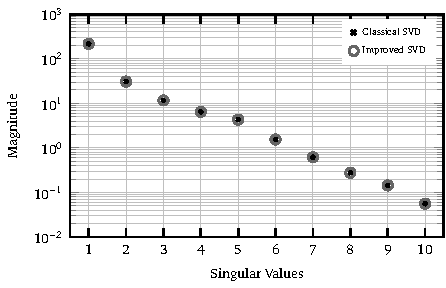
\includegraphics{svd_compare.pdf}
    \caption[Singular values computed by conventional and
    improved \glsfmtshort{svd} methods]{Comparison of singular values computed by the conventional and
        improved \glsfmtshort{svd} methods. Using the new scheme results in
    identical singular values}
    \label{fig:svdcompare}
\end{figure}

\section{Simulation Results and Discussion}\label{sec:Results}

This section provides a quantitative  demonstration of the reduced computational
demand  of the  improved \gls{dra}  scheme by  comparing it  with the  classical
\gls{dra}implementation. The  physical parameters  of the cell  are the  same as
those published in  Fuller~\etal~\cite{Fuller1994}. \Cref{table:simparams} lists
the  parameters used  in  the  \gls{rom} workflow  (same  as  those employed  by
Lee~\etal~\cite{Lee2012a}).

\begin{table}[!htbp]
    \centering
    \caption{Parameters for \gls{rom} Computation}
    \label{table:simparams}
    \begin{tabular}{@{} l l @{}}
        \toprule
		Initial Cell \glsfmtshort{soc}             & \SI{60}{\percent} \\
		Hankel Block Size                          & 8000              \\
		Discrete-Time Model Sample-Rate,~$T_s$     & \SI{1}{\second}   \\
		Number of Electrolyte EigenModes           & 5                 \\
		Continuous-Time Emulation Frequency,~$F_1$ & \SI{128}{\hertz}  \\
		Desired Number of Singular Values          & 10                \\
		\bottomrule
    \end{tabular}
\end{table}

\Cref{fig:memory}  shows a  comparison  of  the memory  usage  of classical  and
improved \gls{dra} methods.  It is evident that the \gls{svd}  step in classical
\gls{dra}  consumes  an  overwhelming  majority  of  the  total  memory  demand,
requiring \approx \SI{100}{\giga\byte} for a Hankel block size of~8000. This can
be a limiting factor  in modelling slow cell dynamics without  access to a large
memory workstation. The improved \gls{dra} method eliminates this bottleneck and
the memory  usage of \gls{svd} step  is negligible. Overall memory  usage of the
improved  \gls{dra} is  dominated by  Markov parameter  computation. Considering
\SI{10}{\giga\byte} of usable \gls{ram}, this means that 60000~Markov parameters
(Hankel Block-size of~30000) can be captured.

\begin{figure}[!htbp]
    \centering
    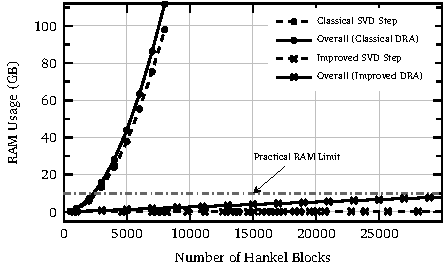
\includegraphics{ram_usage.pdf}
    \caption[%
    Memory usage of classical and improved \glsfmtshort{dra}
    ]%
    {%
        Memory  usage  of  classical and  improved  \glsfmtshort{dra}.  Overall,
        \glsfmtshort{ram}  usage   as  well   as  the   memory  used   only  for
        \glsfmtshort{svd} computation is illustrated.
    }%
    \label{fig:memory}
\end{figure}

\Cref{fig:cputime}  shows   a  comparison  of  \gls{cpu}   times  for  computing
the   \gls{rom}  at   a  single   \gls{soc}   and  temperature   for  both   the
classical  and  the improved  \gls{dra}  methods\footnote{\label{fn:clusterspec}
All  computations  reported  in  this  chapter were  performed  on  a  dedicated
high-\glsfmtshort{ram}  pool  drawn  from  the compute  cluster  hosted  at  the
Department  of  Mathematics at  Imperial  College  London.  The author  of  this
thesis  wishes  to   express  his  thankfulness  to   the  relevant  authorities
for  providing  access  to  this  facility.  The  resources  borrowed  were  one
core  of  a  \mbox{4-core}  \mbox{\text{Intel}\textsuperscript{\textregistered}}
\mbox{Xeon\textsuperscript{\textregistered}} \mbox{E5-2637~v3} processor clocked
at   \SI{3.50}{\giga\hertz}   with   \SI{500}{\giga\byte}   \glsfmtshort{ram}.}.
Owing   to   the   high   operation  count   for   the   \gls{svd}   computation
(see   \cref{eq:cpu_op_count}),  the   classical   \gls{dra}  requires   \approx
\SI{40}{\minute} for a Hankel block size of~8000. Clearly, the overall \gls{cpu}
time for the  classical \gls{dra} is almost exclusively spent  for computing the
\gls{svd}. The improved \gls{dra} method  reduces the overall computational time
by  two  orders of  magnitude,  taking  \approx  \SI{40}{\second} for  the  same
block-size.  In this  case,  the  \gls{cpu} time  is  evenly  split between  the
\gls{svd} and Markov parameter computations.

\begin{figure}[!htbp]
    \centering
    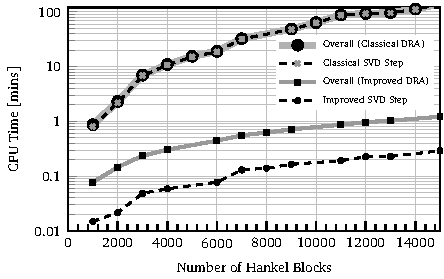
\includegraphics{cpu_usage.pdf}
    \caption{Computation times for classical and improved \glsfmtshort{dra} schemes}
    \label{fig:cputime}
\end{figure}

From  \cref{fig:memory},   it  is  evident   that  if  classical   \gls{dra}  is
employed,  a  standard  laptop  with  a  nominal  \SI{10}{\giga\byte}  \gls{ram}
limit   (dedicated   for   \gls{rom}   workflow)   cannot   capture   the   full
cell   dynamics  and   hence   is  restricted   to   2500~Hankel  blocks.   This
necessitates early  truncation of Markov parameters  at \SI{5000}{\second}. From
\cref{fig:markov_cse_pos}, the truncation residue  at \SI{5000}{\second} for the
unit-pulse response of solid surface concentration at positive current collector
is~$\SI{-0.0087}{\mole\per\meter\cubed}$. The truncation errors in the \gls{mpm}
directly translate  to errors in  computed singular values,  adversely affecting
accuracy of  simulated cell  variables. It  must be noted  that the  accuracy of
simulation results  reported here  does not  bear a  causal relationship  to the
particular  \gls{dra} scheme  employed. In  principle,  when an  upper bound  on
computational usage has not been enforced,  the numerical operations of both the
existing and proposed \gls{dra} schemes lead to similar error magnitudes for the
modelled quantities. Instead, the accuracy comparison illustrated here primarily
serves to demonstrate the practical  usefulness of the improved \gls{dra} scheme
when implemented in a commonplace computing environment.

\Cref{fig:truncated}  shows a  comparison  of singular  values  obtained by  the
classical and improved \gls{svd} methods  computed by imposing a \gls{ram} limit
of \SI{10}{\giga\byte}. Owing to early truncation of the \gls{mpm}, the dominant
singular values  computed by the  conventional method differ  significantly from
those computed by the improved \gls{svd} operating on untruncated data. With the
same memory  constraints, the improved  \gls{dra} can handle up  to 30000~Hankel
blocks, allowing for capture of \SI{60000}{\second} of Markov parameter data.

\begin{figure}[!htbp]
    \centering
    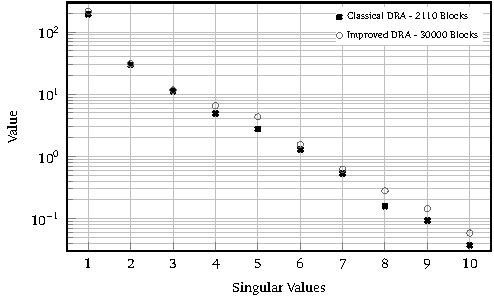
\includegraphics{truncated.pdf}
    \caption{Comparison of singular values computed by conventional and improved
        \glsfmtshort{svd} methods under a practical \glsfmtshort{ram} limit of
    \SI{10}{\giga\byte}}
    \label{fig:truncated}
\end{figure}

For comparative analysis  of modelling accuracy under this  memory constraint, a
time-domain simulation  of the  \glspl{rom} obtained  by classical  and improved
\gls{dra}  methods is  performed.  The input  current  profile corresponding  to
a  \gls{udds}  drive  cycle  reported in  Lee~\etal{}~\cite{Lee2012a}  is  used.
\Cref{fig:time_domain_sim}  depicts  the  time-evolution of  the  solid  surface
concentration  at  the  positive  electrode/separator  boundary.  For  comparing
the  accuracy   of  the   two  ROMs,  a   COMSOL  Multiphysics~\cite{COMSOL2012}
simulation  of  the  full-order   pseudo-2D  porous-electrode  \gls{pdae}  model
is  used  as   the  reference.  The  \gls{rom}   employing  classical  \gls{dra}
diverges  over   time,  and  after   \SI{1500}{\second}  results  in   an  error
of  \SI{1120}{\mole\per\meter\cubed}.   The  \gls{rom}  incorporating   the  new
\gls{dra}  workflow   accurately  tracks   the  COMSOL   simulation  trend-line.

\begin{figure}[!htbp]
    \centering
    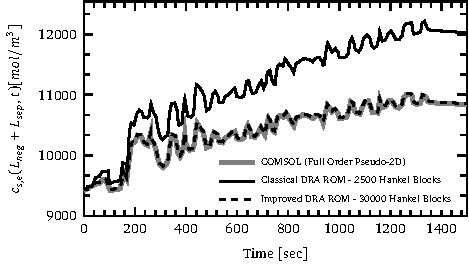
\includegraphics{comsol_comparison.pdf}
    \caption[%
    Evolution of solid surface concentrations at
    positive electrode/separator interface.
    ]%
    {%
        Time-domain  simulation depicting  solid surface  concentrations at  the
        boundary  of positive  electrode and  separator. The  simulation results
        from  the  \gls{p2d}  model  implemented   in  COMSOL  is  used  as  the
        reference  benchmark. The  two  \glsfmtshortpl{rom}  were derived  under
        a  \glsfmtshort{ram}  limit   of  \SI{10}{\giga\byte}.  The  performance
        of  the  improved \glsfmtshort{dra}  is  significantly  better than  the
        classical \glsfmtshort{dra} owing to the  fact that its derivation could
        accommodate  a larger  number  of Hankel  blocks  without exceeding  the
        specified memory limit.
    }%
    \label{fig:time_domain_sim}
\end{figure}

\Cref{tbl:salientresults}   provides   a   summary   of   the   key   simulation
results.  At  a  single  operating  point  of  \gls{soc}  and  temperature,  for
a  Hankel  block   size  of~8000,  the  \gls{rom}   workflow  incorporating  the
improved  \gls{dra}  is  \approx  100  times  faster  than  that  employing  the
classical   \gls{dra}.  Using   the  machine   with  specifications   listed  in
the  footnote\textsuperscript{\ref{fn:clusterspec}},  for  100~operating  points
(combinations of  10~\gls{soc} and temperature values),  computing the \gls{rom}
requires  only  6~hours using  the  improved  \gls{dra}, whereas  the  classical
\gls{dra} consumes  666~hours (27~days).  Furthermore, for the  same block-size,
the  improved \gls{dra}  is  demonstrated  to be  superior  in  terms of  memory
efficiency,  drastically reducing  the memory  requirement from  112~GB down  to
2~GB. Finally,  the improved \gls{dra} demonstrates  superior modelling accuracy
when  implemented even  in moderately  equipped computing  environments such  as
laptops.

\begin{table}[!htbp]
	% \singlespacing
	\centering
	\caption{Salient Results --- Classical vs.\ Improved \gls{dra} }
	\label{tbl:salientresults}
	\setlength{\extrarowheight}{1pt}
	\begin{tabular}{ @{} l c l l @{} }
		\toprule
		% \gls{rom}                                & Quantity                                & Classical                                   & Improved                                  \\
		% Condition                                &                                         & \gls{dra}                                   & \gls{dra}                                 \\
		\makecell{\gls{rom} \\ Condition} & {Entity} & \makecell{Classical \\ \gls{dra} } & \makecell{Improved \\ \gls{dra}} \\
		\midrule
		\multirow{8}{1.22cm}{8000 Hankel Blocks} & Memory                         & 111.80 GB                        & 2.14 GB                        \\ [-5pt]
                                                 & \footnotesize (overall)        &                                  &                                \\
                                                 & Memory                         & 97.93 GB                         & 0.03 GB                        \\ [-5pt]
                                                 & \footnotesize(\gls{svd} step)  &                                  &                                \\
                                                 & \gls{cpu} Time                 & 39.78 min                        & 0.63 min                       \\ [-5pt]
                                                 & \footnotesize(overall)         &                                  &                                \\
                                                 & \gls{cpu} Time                 & 39.30 min                        & 0.14 min                       \\ [-5pt]
                                                 & \footnotesize(\gls{svd} step)  &                                  &                                \\ [2.5pt]
		\midrule
		\multirow{3}{1.22cm}{10 GB Memory Limit} & Block Size                     & 2500                             & 30000                          \\ [5pt]
                                                 & Max.\ error                    & \SI{1120}{\mole\per\meter\cubed} & \SI{13}{\mole\per\meter\cubed} \\ [-5pt]
                                                 & in $c_{{s,e}_\text{pos}}(1,t)$ &                                  &                                \\ [5pt]
		\bottomrule
	\end{tabular}
\end{table}

% The  proposed  method opens  up  the  possibility  of modelling  other  physical
% quantities  in  the   cell's  geometry  without  being   hindered  by  computing
% limitations. Furthermore, high sample-rate models  to handle highly dynamic load
% profiles  can be  deployed in  future  \gls{bms} applications.  The scheme  also
% empowers the \gls{rom} framework to tackle  cells with slower dynamics and other
% chemistries  with different  rate-limiting  mechanisms.  The improved  \gls{dra}
% method therefore  opens up a  wide range of  possibilities and looks  capable of
% bringing  the goal  of  physics-based  battery model  implementation  in a  high
% performance real-time \gls{bms}, a step closer to realisation.

% Despite   the  aforementioned   euphoric   possibilities   facilitated  by   the
% streamlining  of  the reduced  order  modelling  workflow through  the  improved
% \gls{dra},  there  exists a  fundamental  deficiency  in this  hybrid  modelling
% approach  that impede  its  effective deployment  as the  plant  model in  state
% estimation tasks. This aspect was already discussed in \cref{ch:littreview}, and
% is  reiterated here.  The  entries in  the  matrices of  the  final state  space
% model  depend on  the linearisation  point  of \gls{soc}  and temperature.  This
% linearisation requirement adversely affects the usability of the model for state
% estimation tasks, wherein the \gls{soc} is in fact an unknown quantity and is to
% be  estimated.  This  cyclic  dependency between  the  linearisation  point  and
% the  state-estimation quantity  makes  the  use of  this  model questionable  in
% a  demanding  application such  as  in  embedded \glspl{bms}  on-board  electric
% vehicles.

This  chapter  concludes  with  the  view  that,  although  the  bottlenecks  in
Lee~\etal~\cite{Lee2012a}  revealed   by  this   in-depth  analysis   have  been
effectively tackled  in this chapter,  owing to the circular  dependency between
the linearisation point and model parameters, the underlying model itself is not
robust enough for immediate implementation. Furthermore, the model derivation is
convoluted  with the  derivation being  performed  in the  frequency domain  and
implementation in the  time-domain. This thesis author is of  the opinion that a
simple, yet  accurate model derived  and implemented entirely in  time-domain is
the  need  of  the  hour  for  encouraging  the  automotive  industry  to  adapt
physics-based battery models onto on-board  \glspl{bms} of electric vehicles. In
the quest to  fulfil this need, an analysis of  the simplest time-domain physics
based model \viz~the \gls{spm} is presented next in \cref{ch:spmanalysis}.
